\begin{figure*}
    \centering
    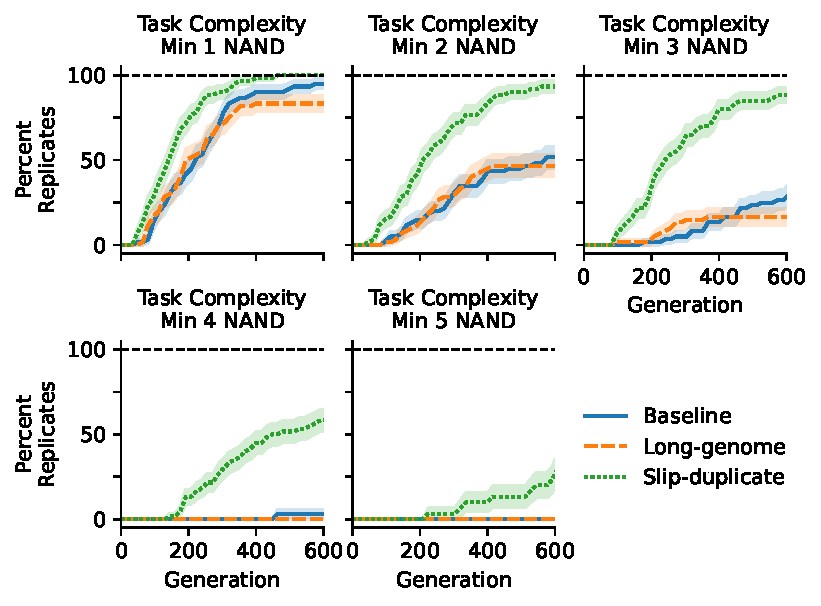
\includegraphics[width=\linewidth]{binder/binder/teeplots/adaptive-evolution-rate.ipynb/col=task-complexity+errorbar=se+hue=treatment+kind=line+mutation=poisson+post=plt-xlim-0-600+style=treatment+viz=relplot+x=generation+y=has-task+ext=.pdf}
    \caption{
        \textbf{Mutational supply drives increased adaptation rate for long-genome control treatment.}
        \footnotesize
           Results shown from supplemental control experiments using per-genome, rather than per-site, point mutation processes.
           In these trials, a count of point mutations was drawn from a Poisson distribution, to be applied at random positions on the genome.
           Mean per-genome mutation rate was configured corresponding with that under per-site mutation for a 100-site genome.
           Plots show fraction of replicates performing logic-9 phenotypes, by generation from founding ancestor.
            Panels facet by logic-9 task complexity, measured by the minimum number of NAND operations required to complete the task.
            Simple tasks (top left) require only one NAND operation.
            More complex tasks require up to five NAND operations (bottom right).
        Compared to Figure \ref{fig:adaptive-evolution-rate}, which shows results with per-site mutation rates, the relative rate of adaptive evolution in long-genome control is diminished under Poisson-distributed treatment, where mutation count is not proportional to genome length.
        Error bands give 95\% CI, bootstrapped over 30 replicates per treatment.
    }
    \label{fig:adaptive-evolution-rate-poisson}
\end{figure*}
